\chapter{Конструкторский раздел}
\label{cha:design}
В данном разделе будут рассмотрены схемы алгоритмов умножения матриц.
На рис. \ref{d:ref1} представлена схема стандартного алгоритма умножения матриц.

\begin{figure}[ht!]
	\centering{
		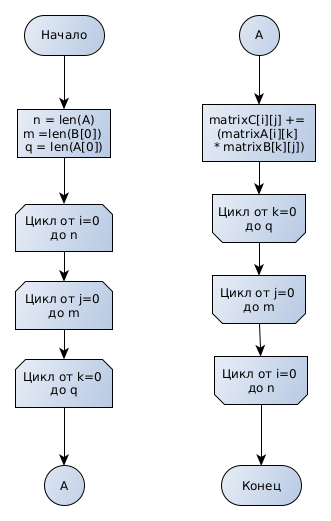
\includegraphics[width=0.6\textwidth]{img/d1.png}
		\caption{Схема стандартного алгоритма умножения матриц}
		\label{d:ref1}}
\end{figure}

На рис. \ref{d:ref2} - \ref{d:ref3} представлена схема алгоритма Винограда умножения матриц .


\begin{figure}[ht!]
	\centering{
		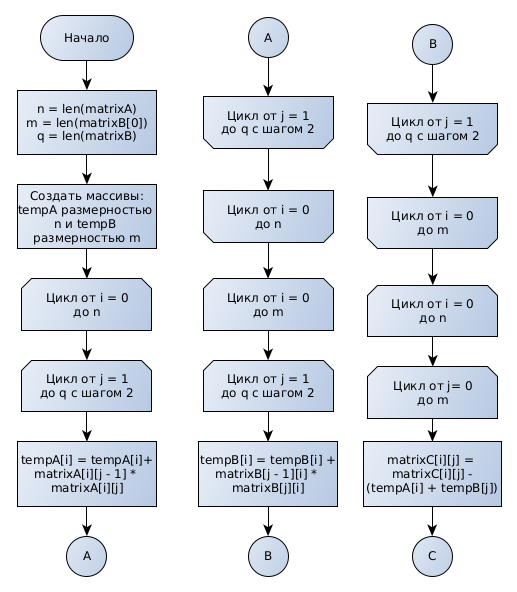
\includegraphics[width=0.7\textwidth]{img/d2.png}
		\caption{Схема алгоритма Винограда умножения матриц}
		\label{d:ref2}}
\end{figure}

\begin{figure}[ht!]
	\centering{
		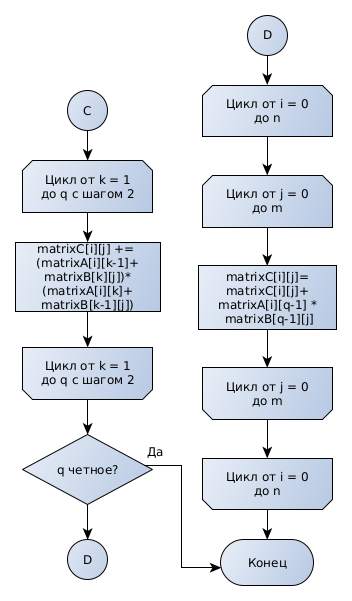
\includegraphics[width=0.5\textwidth]{img/d3.png}
		\caption{Схема алгоритма Винограда умножения матриц}
		\label{d:ref3}}
\end{figure}

\section{Вывод}

В данном разделе были рассмотрены схемы (рис. \ref{d:ref1} - \ref{d:ref3}) алгоритмов умножения матриц.